Neutrino oscillation experiments measure an event rate, which is the convolution of the flux, cross section and detector efficiency, as a function of some measureable variable. The incoming neutrino energy is not known event by event, and not all outgoing particles are detectable, so quantities such as the energy transfer, or four-momentum transfer, cannot be reconstructed. As neutrino oscillation is a neutrino energy (and distance) dependent phenomenon, experiments attempt to reconstruct it using the kinematics of particles produced when neutrinos interact in their detectors.

T2K, and other experiments with a relatively low energy ($\lessapprox1$ GeV) beam~\cite{Hyper-Kamiokande:2018ofw, MiniBooNE:2020pnu}, attempt to reconstruct the neutrino energy using outgoing lepton momentum, $p_{l}$, and its angle with respect to the incoming beam direction, $\theta_{l}$, assuming two-body quasielastic kinematics with the initial nucleon at rest,
\begin{equation}
E^{\mathrm{rec,\;QE}}_{\nu}\left(p_{l}, \theta_{l}\right) = \frac{2m_f\sqrt{p_{l}^2 + m^2_l} - m_l^2 + m_i^2-m_f^{2}}{2\left(m_f-\sqrt{p_{l}^2 + m^2_l}+p_l \cos\theta_l\right)},
\label{eq:enuqe}
\end{equation}
\noindent where $m_l$ is the mass of the outgoing lepton, $m_{i}$ is the mass of the initial state nucleon, and $m_{f}$ is the mass of the final state nucleon. As this variable assumes quasielastic kinematics, it is applied to a signal sample of events with a muon, no pions or other mesons, and any number of nucleons produced in the final state\footnote{Note that in recent analyses, T2K has included samples including a single charged pion using a modified version of Equation~\ref{eq:enuqe}~\cite{T2K:2017rgv, T2K:2019bcf, T2K:2021xwb}.} (CC0$\pi$).%
\begin{marginnote}
\entry{CC0$\pi$}{Events with a muon, no pions or other mesons, and any number of nucleons produced in the final state}
\end{marginnote}%
Events that are not true CCQE events also contribute to the CC0$\pi$ signal, such as charged-current interactions with two nucleons (CC-2p2h) or charged-current interactions with resonant production (CC-RES) but no visible final state pion. The two-body approximation in Equation~\ref{eq:enuqe} is a poor approximation of the true neutrino energy, $E_{\nu}^{\mathrm{true}}$, in these cases. Understanding the relative fraction of the different interaction channels is therefore a critical issue for experiments that use Equation~\ref{eq:enuqe}.

\begin{figure}[htbp]
  \centering
  \captionsetup[subfloat]{captionskip=-5pt}
  \subfloat[Near detector]{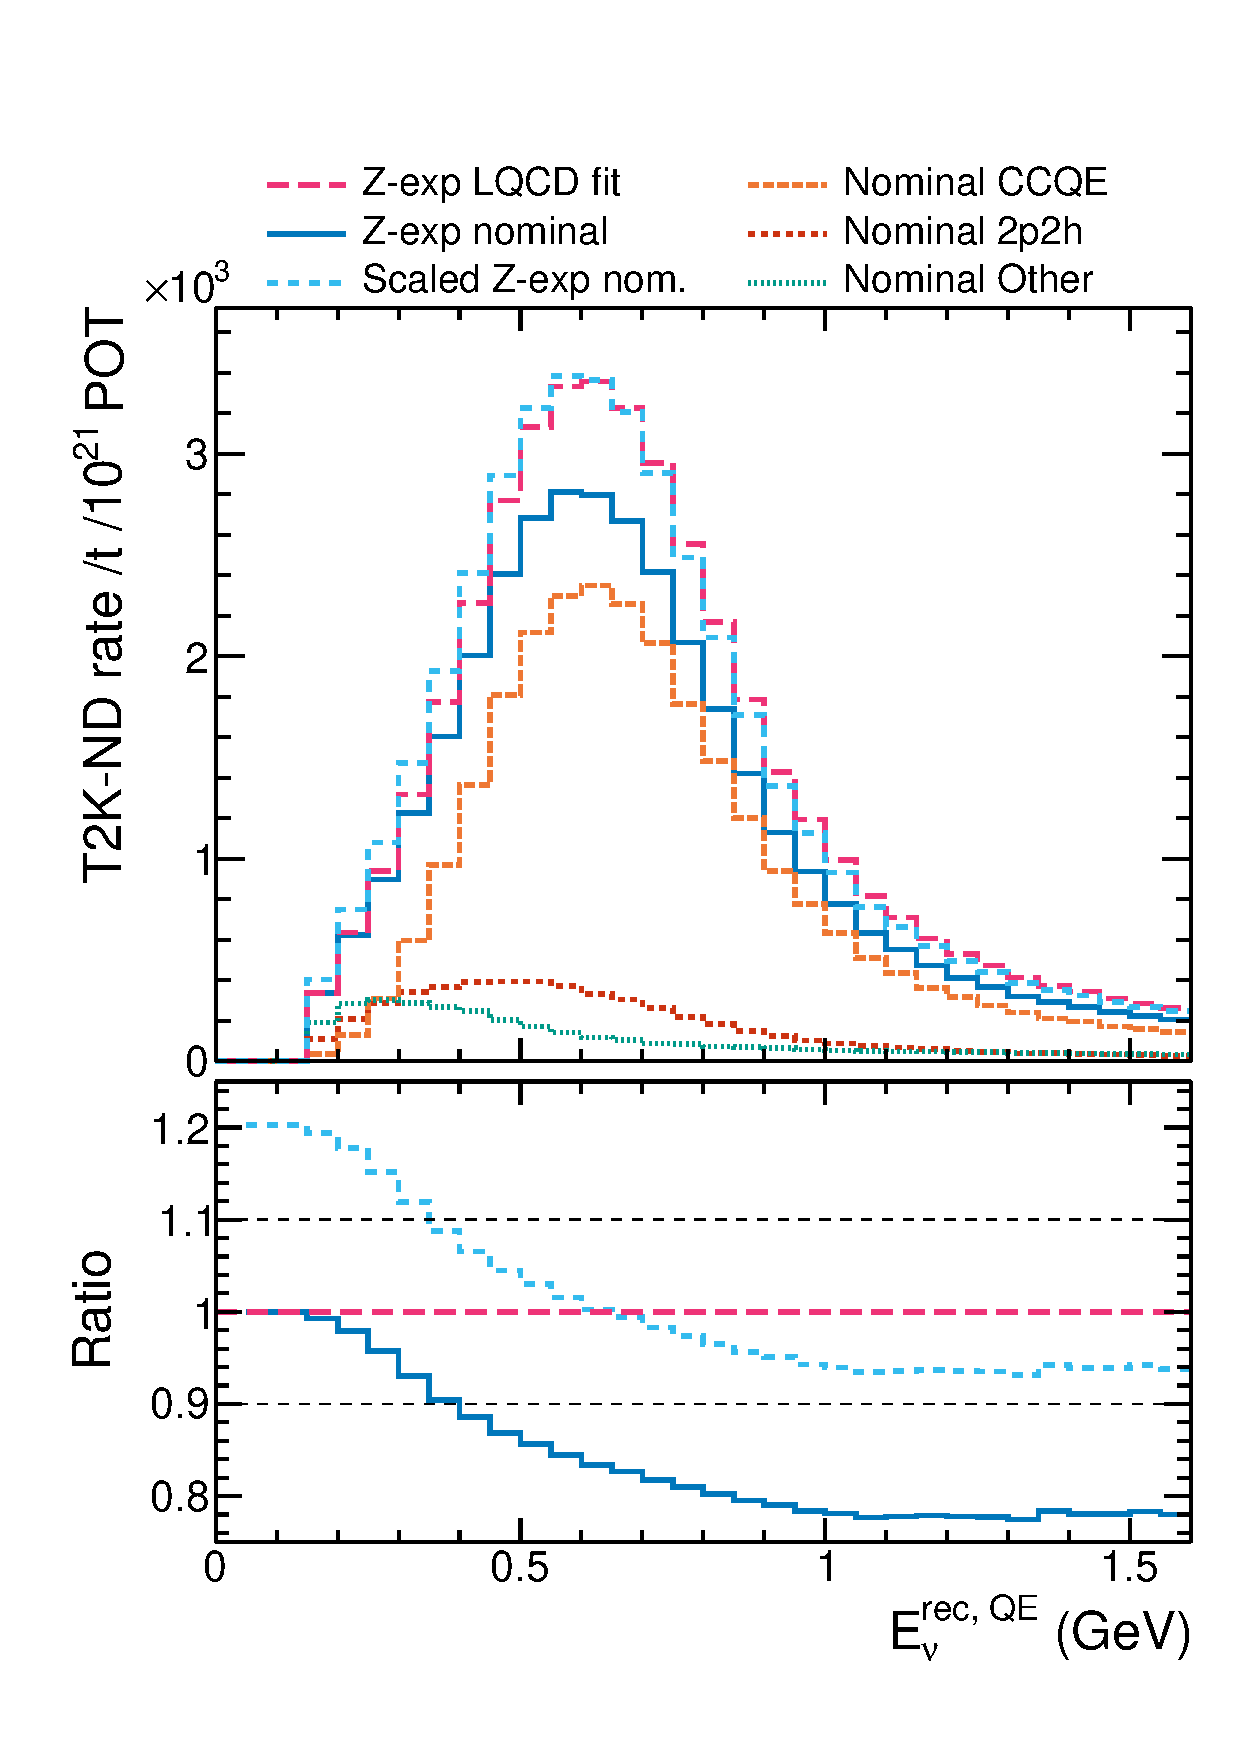
\includegraphics[width=0.3\textwidth]{plots/T2KND_numu_H2O_model_comp.pdf}}\hspace{75pt}
  \subfloat[Far detector] {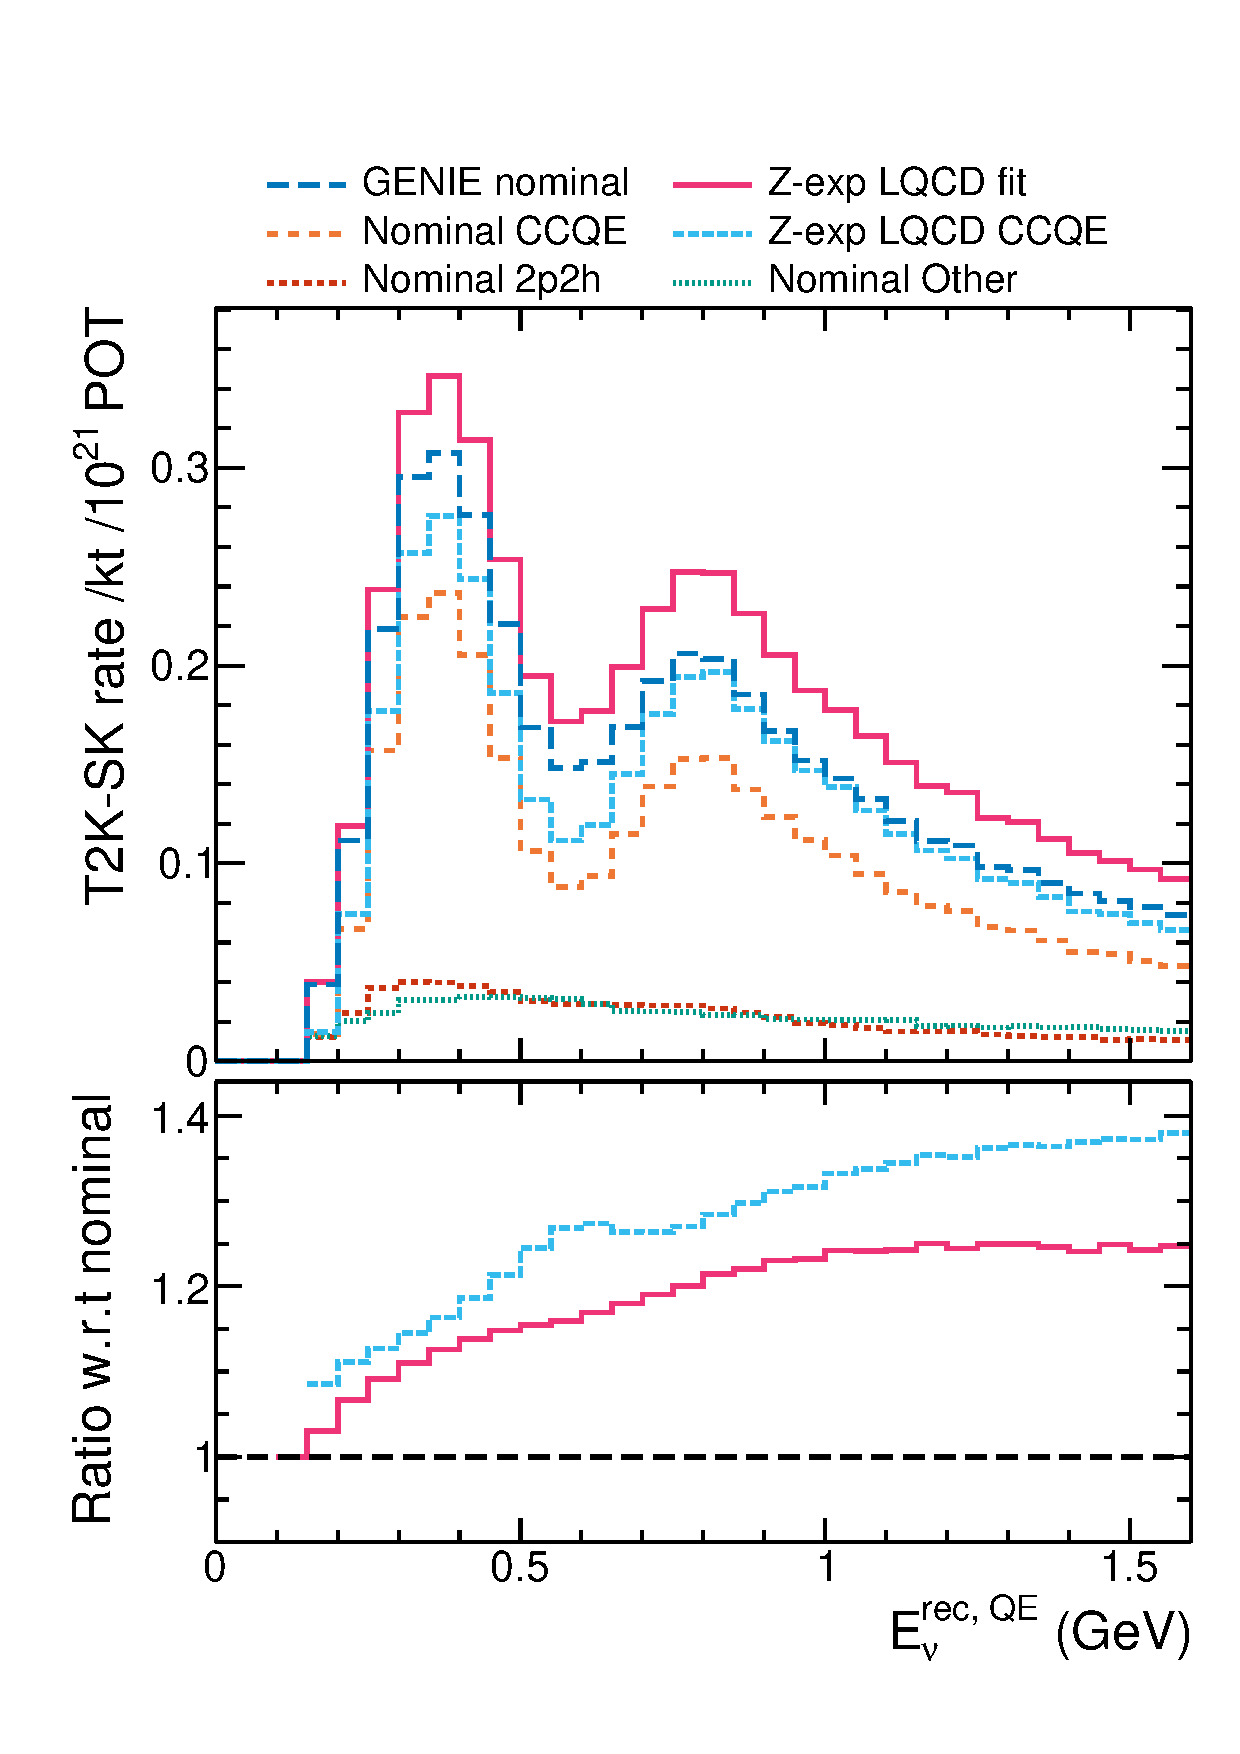
\includegraphics[width=0.3\textwidth]{plots/T2KFD_numu_H2O_osc_model_comp.pdf}}
  \vspace{11pt}
  \caption{The $\nu_{\mu}$--H$_{2}$O CC0$\pi$ event rates per ton (kiloton) per $1\times10^{21}$POT at T2K's near (far) detector site, shown as a function of $E^{\mathrm{rec,\;QE}}_{\nu}$. The GENIE~\cite{Andreopoulos:2009rq, GENIE:2021npt} nominal event rate (blue solid line) is produced using the GENIEv3 10a\_02\_11a tune to nucleon data~\cite{GENIE:2021zuu} and the T2K flux~\cite{T2K:2012bge}, and the CCQE (orange dashed line), CC-2p2h (red short dashed line) and CC-other (green dotted line) contributions are shown. The oscillated flux is calculated using the best fit NuFit5.0 oscillation parameters in normal ordering~\cite{Esteban:2020cvm, nufitweb}. Additionally, an alternative GENIE model is shown, where the only change is to use the z-expansion model of the axial form factor, with parameters tuned to LQCD results, as described in Section~\ref{sec:z_continuum}. \cw{Check this is true with changed section ordering!} Additionally, the ratio of the modified to nominal GENIE models is shown.}
  \label{fig:t2k_impact}
\end{figure}
Figure~\ref{fig:t2k_impact} shows the $\nu_{\mu}$--H$_{2}$O CC0$\pi$ event rate expected at the T2K near and far detectors for a fixed exposure, shown as a function of $E^{\mathrm{rec,\;QE}}_{\nu}\left(p_{l}, \theta_{l}\right)$, with and without modifications to the axial form factor. The nominal GENIEv3 10a\_02\_11a model~\cite{Andreopoulos:2009rq, GENIE:2021npt} uses a dipole axial form factor with $M_{\mathrm{A}} = 0.941$ GeV$^2$ obtained through a fit to bubble chamber data~\cite{GENIE:2021zuu}. The alternative model shown differs only in the use of the z-expansion model for the axial form factor, with parameters tuned to the LQCD results described in Section~\ref{sec:z_continuum}. One obvious observation to be made from Figure~\ref{fig:t2k_impact} is that the CCQE events which the axial form factor is relevant for clearly make up the majority of T2K's CC0$\pi$ sample, in both the oscillated and unoscillated fluxes. It is also clear that the tuned LQCD value has significant effect on the total expected event rate in both cases, on the order of 20\%.

Also clear from Figure~\ref{fig:t2k_impact} is that the change in the total, or CCQE-contributed event rates is not purely a normalization change, and is different for the near and far detector spectra. In the T2K oscillation analysis, the near detector data is used to constrain the cross-section model, to reduce the uncertainty at the far detector and on the measured oscillation parameters. If there is insufficient freedom in the cross-section model to account for this change to the CCQE model, other parts of the model may well be distorted to ensure good agreement with the near detector data. However, this can introduce biases at the far detector, as the different interaction types that contribute to the CC0$\pi$ samples shown in Figure~\ref{fig:t2k_impact} have very different $E_{\nu}^{\mathrm{true}}$ --- $E^{\mathrm{rec,\;QE}}_{\nu}$ relationships. So if other components of the model are distorted to fit the unoscillated near detector event rate, that same {\it effective} change is not in general expected to extrapolate to the far detector spectrum correctly.

Experiments with higher neutrino beam energies typically do not limit their analyses to CC0$\pi$ events or use Equation~\ref{eq:enuqe} for reconstructing the neutrino energy. Instead, they use all charged-current events (CC-inclusive), and reconstruct the neutrino energy through a combination of particle identification and tracking, and calorimetry. For an ideal detector, with no tracking threshold on protons, charged pions or electromagnetic activity, this can be expressed as,
\begin{equation}
E_{\nu}^{\mathrm{rec,\;had}} = E_{l} + \Sigma_{p} E_{\mathrm{kin}} + \Sigma_{\pi^{\pm}, \pi^{0}, \gamma} E_{\mathrm{total}},
\label{eq:enuhad}
\end{equation}
\noindent where $E_{l}$ is the energy of the outgoing charged lepton. The $E_{\nu}^{\mathrm{true}}$ --- $E_{\nu}^{\mathrm{rec,\;had}}$ smearing in this idealized case is due to missing kinetic energy lost to neutrons, and initial state nuclear effects (e.g., nucleons are not at rest inside the nucleus). Real detectors have tracking thresholds below which charged particles cannot be reconstructed, which results in additional smearing due to missing the masses of charged pions, although some energy lost to neutrons may be recovered.

\begin{figure}[htbp]
  \centering
  \subfloat[ND]{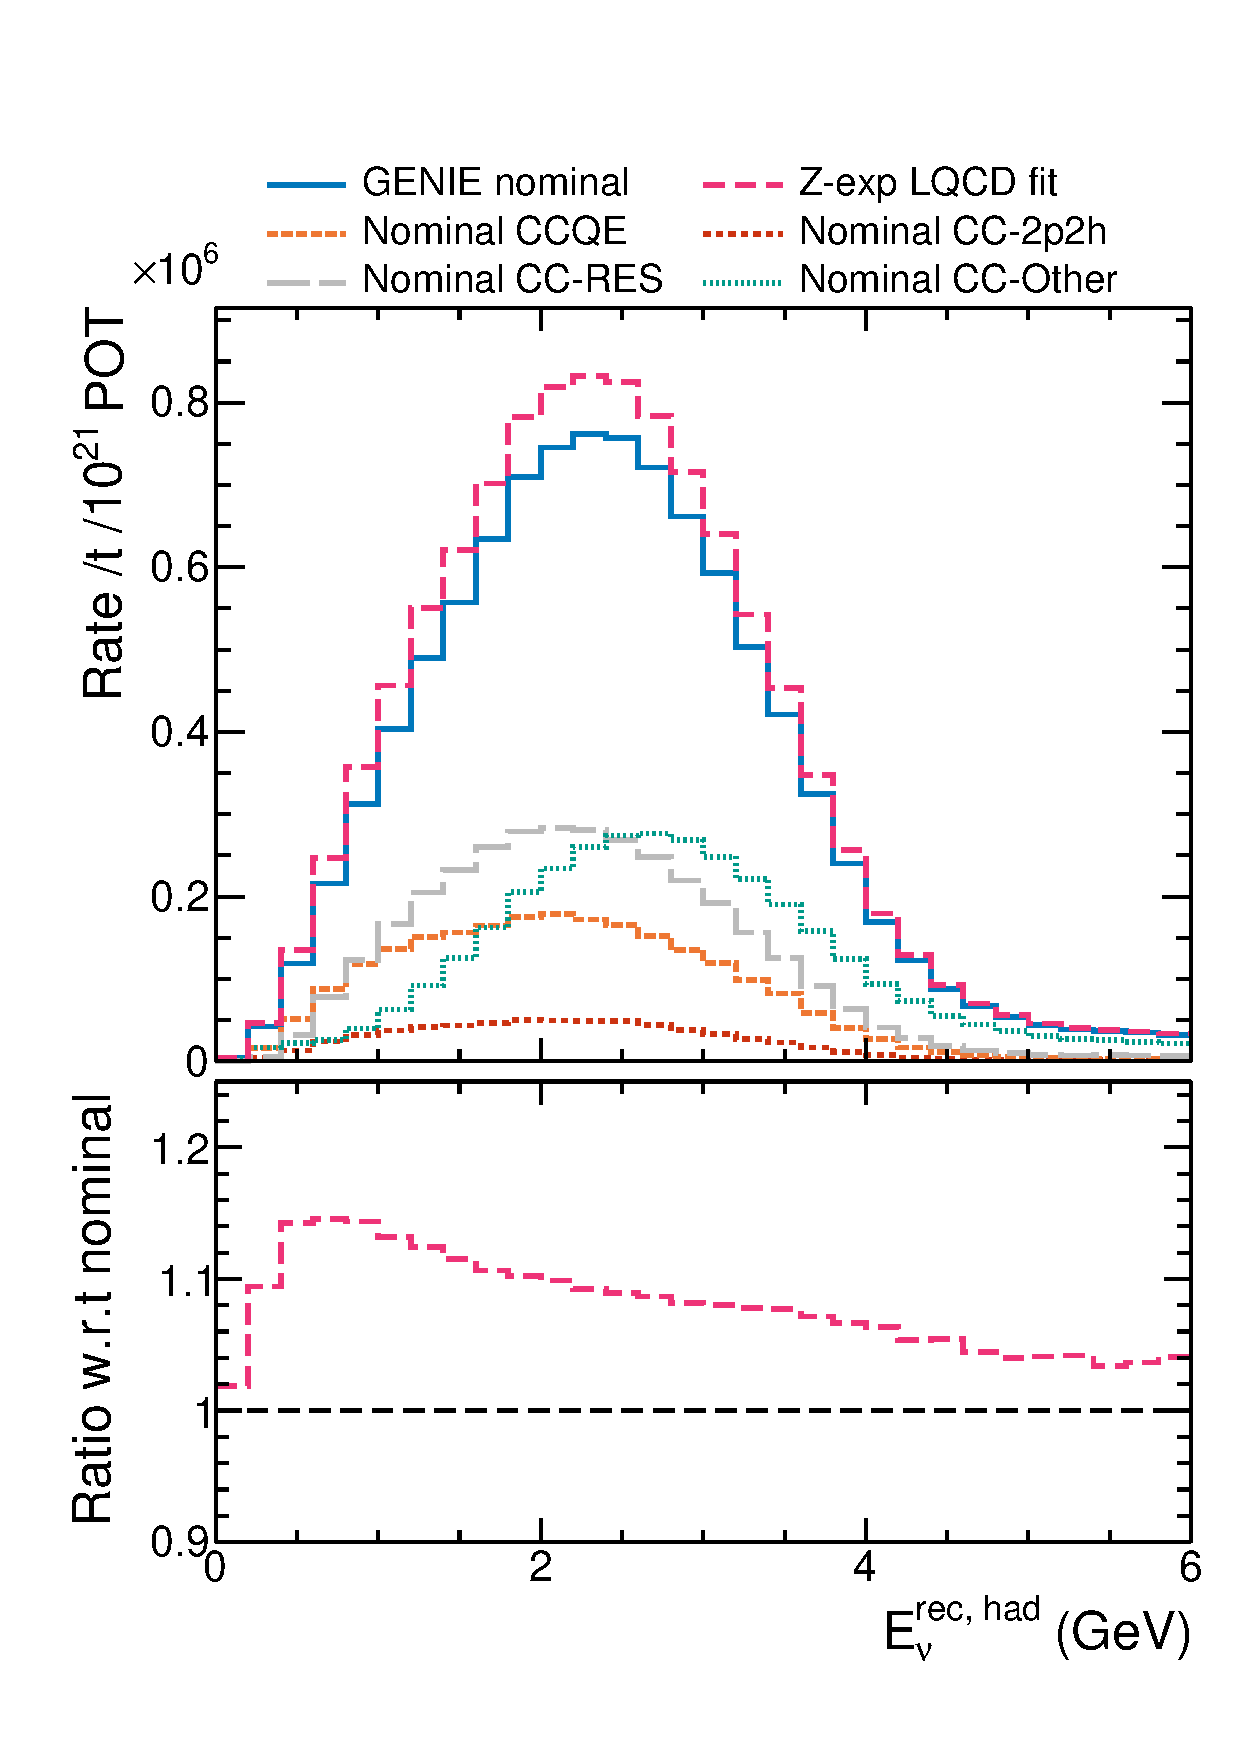
\includegraphics[width=0.3\textwidth]{plots/DUNE_numu_Ar40_breakdown.pdf}}\hspace{75pt}
  \subfloat[FD]{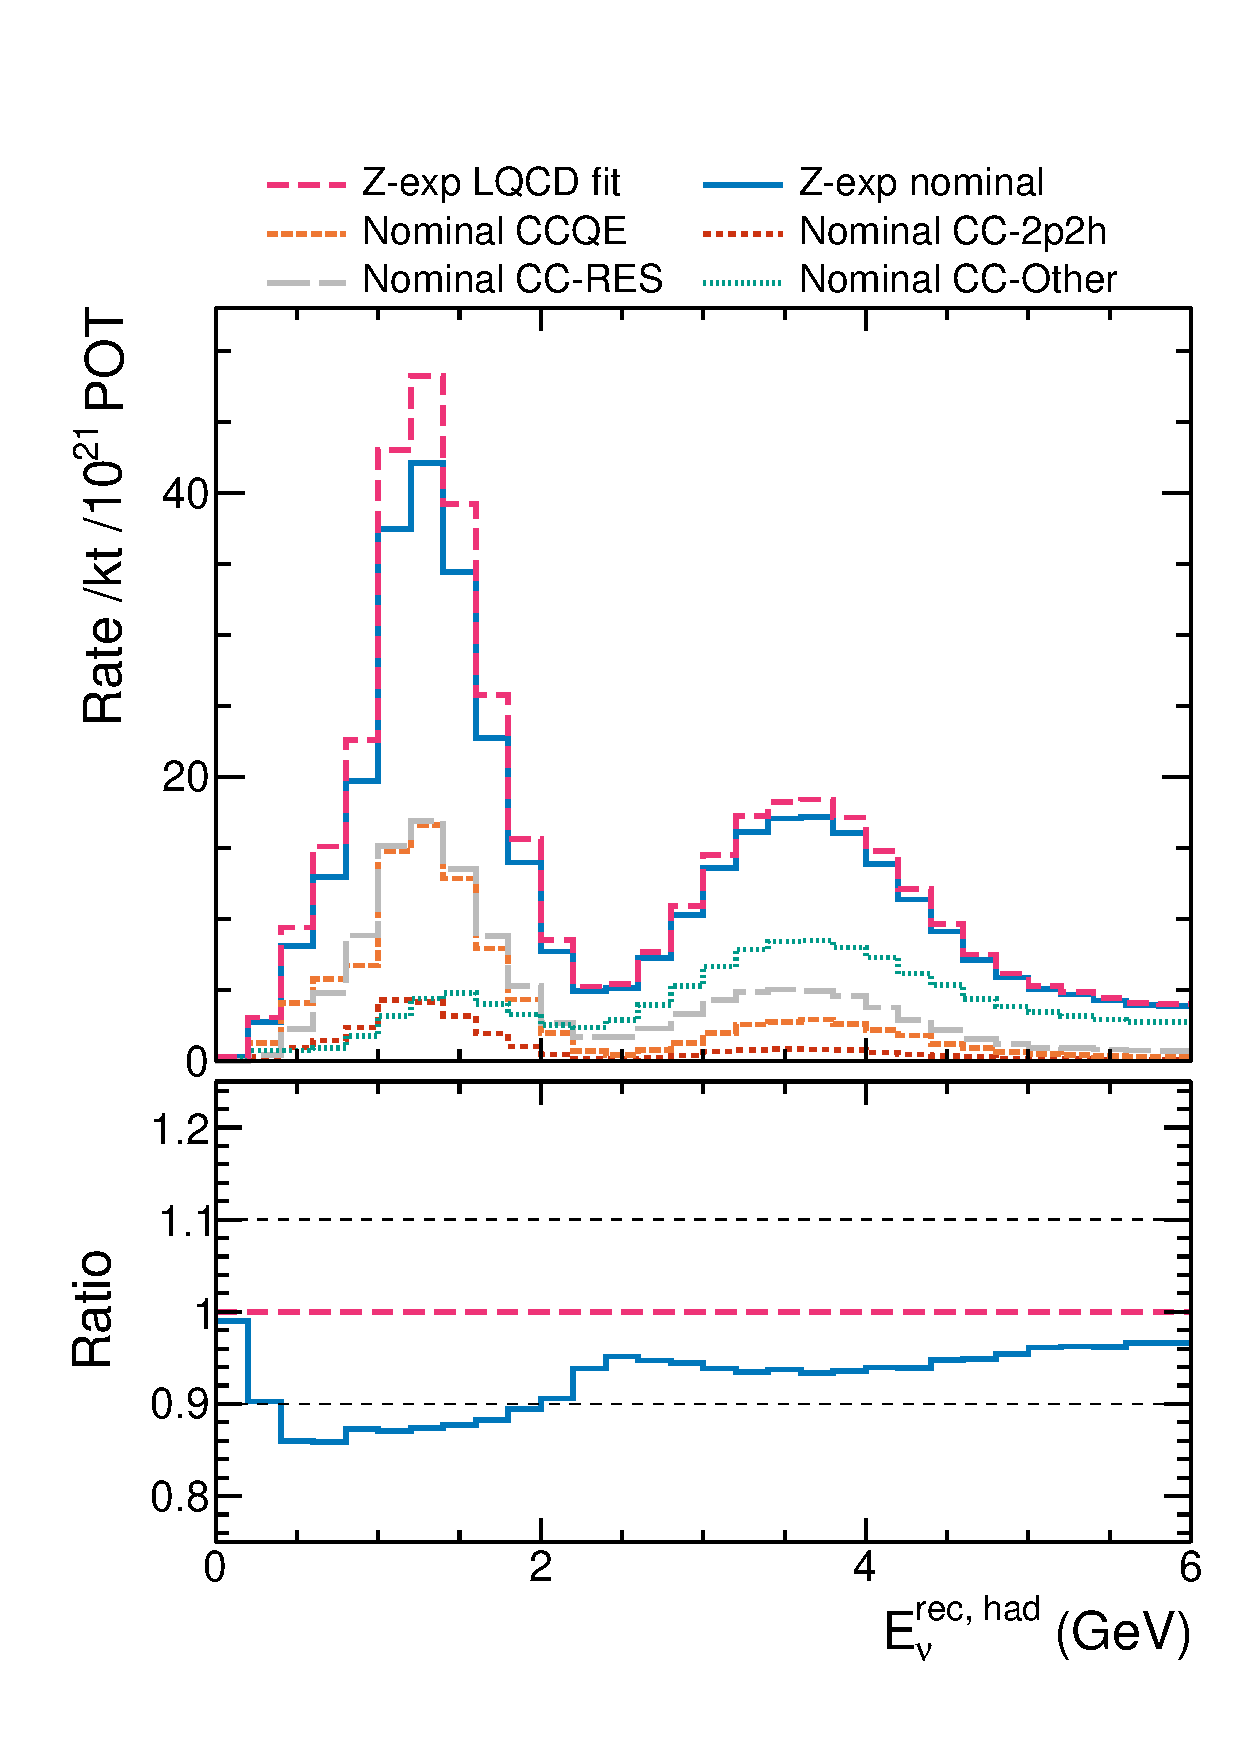
\includegraphics[width=0.3\textwidth]{plots/DUNE_osc_numu_Ar40_breakdown.pdf}}
  \vspace{11pt}
  \caption{The $\nu_{\mu}$--$^{40}$Ar CC-inclusive event rates per ton (kiloton) per $1\times10^{21}$POT at DUNE's near (far) detector site, shown as a function of $E^{\mathrm{rec,\;had}}_{\nu}$. The GENIE~\cite{Andreopoulos:2009rq, GENIE:2021npt} nominal event rate (blue solid line) is produced using the GENIEv3 10a\_02\_11a tune to nucleon data~\cite{GENIE:2021zuu} and the DUNE flux~\cite{Abi:2020evt}, and the CCQE (orange dashed line), CC-2p2h (red short dashed line), CC-RES (long-dashed gray line) and CC-other (green dotted line) contributions are shown. The oscillated flux is calculated using the best fit NuFit5.0 oscillation parameters in normal ordering~\cite{Esteban:2020cvm, nufitweb}. Additionally, an alternative GENIE model is shown, where the only change is to use the z-expansion model of the axial form factor, with parameters tuned to LQCD results, as described in Section~\ref{sec:z_continuum}. \cw{Check this is true with changed section ordering!} Additionally, the ratio of the modified to nominal GENIE models is shown.}
  \label{fig:dune_impact}
\end{figure}
Figure~\ref{fig:dune_impact} shows the $\nu_{\mu}$--$^{40}$Ar CC-inclusive event rates per ton (kiloton) per $1\times10^{21}$POT at DUNE's near (far) detector site, shown as a function of $E^{\mathrm{rec,\;had}}_{\nu}$, with and without modifications to the axial form factor. At this higher neutrino beam energy (with $E_{nu}^{\mathrm{peak}} \approxeq 2.5$ GeV), CCQE events still make up a sizeable, $\approx$30\%, fraction of the total events. The modification to the axial form factor based on the LQCD results described in Section~\ref{sec:z_continuum} has an approximately 10\% effect to the total predicted event rate at both the near and far detectors, with different shape dependence, as in the T2K case. Despite the different neutrino energy reconstruction methods used by DUNE and T2K, the same arguments about potential bias due to model-dependence apply when there are differences in the effect of an out-of-model change between near and far detectors.

\new{The issue of how to assign strength between the CCQE and CC-2p2h channels has been a major focus for neutrino oscillation experiments over the past decade. Experimental data from a large number of experiments has found disagreements on the 10--30\% level between model predictions and data in the CC$0\pi$ channel~\cite{garvey_review_2014, Mosel:2016cwa, NuSTEC:2017hzk, Katori:2016yel, ParticleDataGroup:2020ssz}, prompting development of {\it ad hoc} systematic uncertainties and empirical model tunings by individual experiments, with a tendancy has been to soak up model-data discrepancies into the CC-2p2h channel. These are major contributors to the final uncertainties on key oscillation parameter measurements and projected sensitivities~\cite{T2K:2019bcf, DUNE:2020jqi, T2K:2021xwb, NOvA:2021nfi, DUNE:2021mtg}. It is therefore very significant that the LQCD results shown in Figures~\ref{fig:t2k_impact} and~\ref{fig:dune_impact} suggest that an increase to the strength of the CCQE contribution on the order of 20\% is necessary.}
